\documentclass[thesis.tex]{subfiles}

\begin{document}

\begin{align}
  \beta^{-}\ \text{decay}&:    &   n\ &\longrightarrow\ p + e^{-} + \bar{\nu}_{e} \\
  \beta^{+}\ \text{decay}&:    &   p\ &\longrightarrow\ n + e^{+} + \nu_{e} \\
  \text{Electron capture}&:  &   p + e^{-}\ &\longrightarrow\ n + \nu_{e}
\end{align}

\begin{table}
  \centering
  \begin{tabular}{ l @{\hskip 50pt} l @{\hskip 50pt} l } \hline
    Decay Type     & $\Delta J = J_{F} - J_{I}$ & $\pi_{F}\pi_{I}$ \\ \hline\hline
    Fermi          & 0                         & +1 \\
    Gamow-Teller   & $1    (J_{F}=0\ \text{or}\ J_{I}=0)$   & +1 \\
    Gamow-Teller   & $0,1  (J_{F}>0\ \text{and}\ J_{I}>0)$  & +1 \\ \hline
  \end{tabular}
  \caption{Single-particle states and their quantum numbers and their energies from Eq.~(\ref{eq:pairingsp}). The degeneracy for every quantum number $p$ is equal to 2 due to the two possible spin values.}
  \label{tab:pairingmodelsp}
\end{table}

\begin{figure}
  \centering
  \begin{subfigure}{0.5\linewidth}
    \centering
    \hspace{1.1cm}
    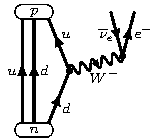
\includegraphics[height=3.5cm]{betadecay/BetaDecay-figure0.pdf}
  \end{subfigure}
  \hspace{-0.25\linewidth}
  \begin{subfigure}{0.5\linewidth}
    \centering
    \hspace{1.1cm}
    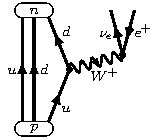
\includegraphics[height=3.5cm]{betadecay/BetaDecay-figure1.pdf}
  \end{subfigure}
\end{figure}

\begin{figure}
  \centering
  \begin{subfigure}{0.5\linewidth}
    \centering
    \hspace{1.1cm}
    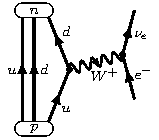
\includegraphics[height=3.5cm]{betadecay/BetaDecay-figure2.pdf}
  \end{subfigure}
  \hspace{-0.225\linewidth}
  \begin{subfigure}{0.5\linewidth}
    \centering
    \hspace{1.1cm}
    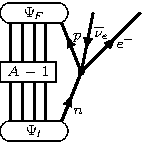
\includegraphics[height=3.5cm]{betadecay/BetaDecay-figure3.pdf}
  \end{subfigure}
\end{figure}

\begin{figure}
  \centering
  \begin{subfigure}{0.5\linewidth}
    \centering
    \hspace{1.0cm}
    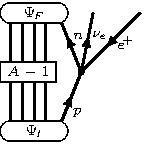
\includegraphics[height=3.5cm]{betadecay/BetaDecay-figure4.pdf}
  \end{subfigure}
  \hspace{-0.175\linewidth}
  \begin{subfigure}{0.5\linewidth}
    \centering
    \hspace{1.0cm}
    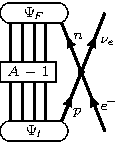
\includegraphics[height=3.5cm]{betadecay/BetaDecay-figure5.pdf}
  \end{subfigure}
\end{figure}



\section{Sum Rules}

\begin{gather}
  \sum_{F} \left[ B_{F_{-}}^{I,F} - B_{F_{-}}^{I,F} \right] = \sum_{F} \left[ \lvert \bra{F}\sum_{i}\tau_{i}^{-}\ket{I} \rvert^{2} - \lvert \bra{F}\sum_{i}\tau_{i}^{+}\ket{I} \rvert^{2} \right] \notag \\
  = \sum_{F} \left[ \bra{I}\sum_{i}\tau_{i}^{+}\ket{F}\bra{F}\sum_{i}\tau_{i}^{-}\ket{I} - \bra{I}\sum_{i}\tau_{i}^{-}\ket{F}\bra{F}\sum_{i}\tau_{i}^{+}\ket{I} \right] \notag \\
  = \bra{I} (\sum_{i}\tau_{i}^{+}) (\sum_{j}\tau_{j}^{-}) - (\sum_{i}\tau_{i}^{-}) (\sum_{j}\tau_{j}^{+}) \ket{I} = \bra{I} 2\sum_{i}\tau_{i}^{z} \ket{I} = \left( N_{I} - Z_{I} \right)
\end{gather}

\begin{gather}
  \sum_{F} \left[ B_{GT_{-}}^{I,F} - B_{GT_{-}}^{I,F} \right] = \sum_{F,\mu} \left[ \lvert \bra{F}\sum_{i}\sigma_{i}^{\mu}\tau_{i}^{-}\ket{I} \rvert^{2} - \lvert \bra{F}\sum_{i}\sigma_{i}^{\mu}\tau_{i}^{+}\ket{I} \rvert^{2} \right] \notag \\
  = \sum_{F,\mu} \left[ \bra{I}\sum_{i}\sigma_{i}^{\mu}\tau_{i}^{+}\ket{F}\bra{F}\sum_{i}\sigma_{i}^{\mu}\tau_{i}^{-}\ket{I} - \bra{I}\sum_{i}\sigma_{i}^{\mu}\tau_{i}^{-}\ket{F}\bra{F}\sum_{i}\sigma_{i}^{\mu}\tau_{i}^{+}\ket{I} \right] \notag \\
  = \sum_{\mu} \left[ \bra{I} (\sum_{i}\sigma_{i}^{\mu}\tau_{i}^{+}) (\sum_{j}\sigma_{i}^{\mu}\tau_{j}^{-}) - (\sum_{i}\sigma_{i}^{\mu}\tau_{i}^{-}) (\sum_{j}\sigma_{i}^{\mu}\tau_{j}^{+}) \ket{I} \right] \notag \\
  = \sum_{\mu} \left[ \bra{I} \sum_{i}\sigma_{i,\mu}^{2}\left( \tau_{i,+}\tau_{i,-} - \tau_{i,-}\tau_{i,+} \right) \ket{I} \right] = 3\ \bra{I} \sum_{i}\left( \tau_{i,+}\tau_{i,-} - \tau_{i,-}\tau_{i,+} \right) \ket{I} \notag \\
  = 3\ \bra{I} 2\sum_{i}\tau_{i}^{z} \ket{I} = 3\left( N_{I} - Z_{I} \right)
\end{gather}

\begin{gather}
  \sum_{F} \left[ B_{F_{-}}^{I,F} - B_{F_{-}}^{I,F} \right] = \left( N_{I} - Z_{I} \right) \\
  \sum_{F} \left[ B_{GT_{-}}^{I,F} - B_{GT_{-}}^{I,F} \right] = 3\left( N_{I} - Z_{I} \right)
\end{gather}


\section{Calculating Beta-Decay Matrix Elements}

Fix these!!!!!!!
\begin{equation}
  \mathcal{M}_{\text{F}} \equiv \relement{\mathcal{F}}{\mathbf{\tau}}{\mathcal{I}} = \delta_{J_\mathcal{F}J_{\mathcal{I}}}\sum_{pq}\relement{p}{\mathbf{\hat{\tau}}}{q}\relement{\mathcal{F}}{\co{p}\ao{q}}{\mathcal{I}}
\end{equation}
\begin{equation}
  \mathcal{M}_{\text{GT}} \equiv \relement{\mathcal{F}}{\mathbf{\sigma\tau}}{\mathcal{I}} = \sum_{pq}\relement{p}{\mathbf{\hat{\sigma}\hat{\tau}}}{q}\relement{\mathcal{F}}{\co{p}\ao{q}}{\mathcal{I}}
\end{equation}

\begin{equation}
  \relement{p}{\mathbf{\hat{\tau}}}{q} = \delta_{n_{p}n_{q}}\delta_{l_{p}l_{q}}\delta_{j_{p}j_{q}}\delta_{t_{p}t_{q}\pm 1}\ \hat{j}_{p}
\end{equation}
\begin{equation}
  \relement{p}{\mathbf{\hat{\sigma}\hat{\tau}}}{q} = \sqrt{6}\ \delta_{n_{p}n_{q}}\delta_{l_{p}l_{q}}\delta_{t_{p}t_{q}\pm 1}\ \hat{j}_{p}\hat{j}_{q}\mathop{(-1)^{l_{p}+j_{p}+\frac{3}{2}}}\sixj{\frac{1}{2}}{\frac{1}{2}}{1}{j_{q}}{j_{p}}{l_{p}}
\end{equation}


\begin{equation}
  B_{\text{F}} \equiv \frac{g^{2}_{\text{V}}}{\hat{J}^{2}_{\mathcal{I}}}\lvert\mathcal{M}_{\text{F}}\rvert^{2}
\end{equation}
\begin{equation}
  B_{\text{F}} = \frac{g^{2}_{\text{V}}}{\hat{J}^{2}_{\mathcal{I}}}\sum_{\mathcal{F}\mathcal{I}}\frac{\element{\Lop^{\mathcal{I}}}{\mathbf{\tau}}{\Rop^{\mathcal{F}}}\element{\Lop^{\mathcal{F}}}{\mathbf{\tau}}{\Rop^{\mathcal{I}}}}{\braket{J_{\mathcal{I}}M_{\mathcal{I}};\lambda-\mu}{J_{\mathcal{F}}M_{\mathcal{F}}}^{2}}
\end{equation}


\begin{equation}
  B_{\text{GT}} \equiv \frac{g^{2}_{\text{A}}}{\hat{J}^{2}_{\mathcal{I}}}\lvert\mathcal{M}_{\text{GT}}\rvert^{2}
\end{equation}
\begin{equation}
  B_{\text{GT}} = \frac{g^{2}_{\text{A}}}{\hat{J}^{2}_{\mathcal{I}}}\sum_{\mathcal{F}\mathcal{I}}\frac{\element{\Lop^{\mathcal{I}}}{\mathbf{\sigma\tau}}{\Rop^{\mathcal{F}}}\element{\Lop^{\mathcal{F}}}{\mathbf{\sigma\tau}}{\Rop^{\mathcal{I}}}}{\braket{J_{\mathcal{I}}M_{\mathcal{I}};\lambda-\mu}{J_{\mathcal{F}}M_{\mathcal{F}}}^{2}}
\end{equation}


\begin{gather}
  B_{\beta^{-}} = \element{\Ref}{\Lop^{n}\mathop{(\mathbf{\hat{\beta^{-}}})^{\dagger}}\Rop^{p}}{\Ref}\element{\Ref}{\Lop^{p}\mathbf{\hat{\beta^{-}}}\Rop^{n}}{\Ref} \\
  B_{\beta^{-}} = \element{\Ref}{\Lop_{p}\mathop{(\mathbf{\hat{\beta^{-}}})^{\dagger}}\Rop_{n}}{\Ref}\element{\Ref}{\Lop_{n}\mathbf{\hat{\beta^{-}}}\Rop_{p}}{\Ref} \\
  B_{\beta^{-}} = \element{\Ref}{\Lop^{n}_{p}\mathop{(\mathbf{\hat{\beta^{-}}})^{\dagger}}\Rop_{0}}{\Ref}\element{\Ref}{\Lop_{0}\mathbf{\hat{\beta^{-}}}\Rop^{n}_{p}}{\Ref} \\
  B_{\beta^{-}} = \element{\Ref}{\Lop_{0}\mathop{(\mathbf{\hat{\beta^{-}}})^{\dagger}}\Rop^{p}_{n}}{\Ref}\element{\Ref}{\Lop^{p}_{n}\mathbf{\hat{\beta^{-}}}\Rop_{0}}{\Ref}
\end{gather}


\begin{gather}
  B_{\beta^{+}} = \element{\Ref}{\Lop^{p}\mathop{(\mathbf{\hat{\beta^{+}}})^{\dagger}}\Rop^{n}}{\Ref}\element{\Ref}{\Lop^{n}\mathbf{\hat{\beta^{+}}}\Rop^{p}}{\Ref} \\
  B_{\beta^{+}} = \element{\Ref}{\Lop_{n}\mathop{(\mathbf{\hat{\beta^{+}}})^{\dagger}}\Rop_{p}}{\Ref}\element{\Ref}{\Lop_{p}\mathbf{\hat{\beta^{+}}}\Rop_{n}}{\Ref} \\
  B_{\beta^{+}} = \element{\Ref}{\Lop^{p}_{n}\mathop{(\mathbf{\hat{\beta^{+}}})^{\dagger}}\Rop_{0}}{\Ref}\element{\Ref}{\Lop_{0}\mathbf{\hat{\beta^{+}}}\Rop^{p}_{n}}{\Ref} \\
  B_{\beta^{+}} = \element{\Ref}{\Lop_{0}\mathop{(\mathbf{\hat{\beta^{+}}})^{\dagger}}\Rop^{n}_{p}}{\Ref}\element{\Ref}{\Lop^{n}_{p}\mathbf{\hat{\beta^{+}}}\Rop_{0}}{\Ref}
\end{gather}


Quenching \cite{HARDY2005,TOWNER2008,KUBODERA1978,OSET1979}


\end{document}
